% Project Lab 2 LaTeX Document
% Version 1.0
\documentclass{article}
\usepackage{listings}
\usepackage[margin=1in]{geometry}
\usepackage{graphicx}
\usepackage{textcomp}
%\usepackage{xcolor,colortbl}
\usepackage[table]{xcolor}
\usepackage{longtable}
\usepackage{caption}
\usepackage{fancyvrb}
\usepackage{placeins}
\usepackage[pdftex,
            pdfauthor={Paul Fortier, Daniel Noyes},
            pdftitle={Project Lab \#3 - Spring 2016 },
            pdfsubject={ECE 368 Digital Design},
            pdfkeywords={Digital Design, VHDL, Nexys 2, Xilinx, ISE},
            pdfproducer={Latex},
            pdfcreator={pdflatex}]{hyperref}


\captionsetup[table]{justification=centering}

%Remove the number display for each section tag
\makeatletter
\renewcommand\@seccntformat[1]{}
\makeatother

%Define gray center for a table
\definecolor{Gray}{gray}{0.85}
\newcolumntype{g}{>{\columncolor{Gray}}c}
%Quick command for multiple lines in a table cell
\newcommand{\specialcell}[2][l]{%
  \begin{tabular}[#1]{@{}l@{}}#2\end{tabular}}


\begin{document}

\begin{center}
\textsc{\huge ECE 368 Digital Design - Spring 2016}\\[1cm]
\textsc{{\LARGE Project Lab \#3: (100pts)}}\\[0.5cm]
\textsc{\Large Lab dates: April $15$\textsuperscript{th}, April $22$\textsuperscript{nd}, and April $29$\textsuperscript{th},2016}\\[0.5cm]
\textsc{\Large Lab Report Due: Wednesday May $13$\textsuperscript{th},2015}\\[1cm]
\end{center}

\section{Overview and Objectives:}
In this laboratory assignment, you will use the Xilinx ISE software tools aimed at the Digilent NEXYS2 Board to expand the ISA for the UMD RISC 16 machine to include LWVI, SWVI, LWVS, SWED, SWEI and INT instructions. This will require the addition of new components in the data path and control path to support these instructions. In particular you will minimally need to add in an external memory unit, a four element set of registers to support the extended memory instructions and additional control elements to manage operations of the new instructions. You must test the completed design using self-written instruction sequences described in your test plan and physically demonstrated and documented in your test plans experimental results (actual measurements).

In this lab, we will expand on the design achieved in Project Lab 1 and Project Lab 2 to realize the high level RISC Harvard Architecture shown in figure~\ref{fig:harvardarc}.

\begin{figure}[!htbp]
  \centering
    \fbox{\includegraphics[width=0.7\textwidth]{images/HarvardArch.png}}
  \caption{Harvard Architecture}
  \label{fig:harvardarc}
\end{figure}
\FloatBarrier

\section{Introduction}

In Project Lab 1 and 2, you minimally implemented an operational 16 bit pipelined RISC machine supporting the basic instructions from the ISA provided. The implemented RISC machine also was integrated with your debug unit supporting input and output control through the keyboard and data and control status information using the VGA from the earlier labs. 

The completed design and architecture is important to properly realize a fully operational UMD RISC-16 machine and ISA. The external memory unit lies outside the core RISC machine and would be considered the next tier in a computer’s memory hierarchy. The core RISC architecture supports high speed registers, localized data and instruction memory (a form of cache memory) and external memory (sometimes referred to as primary memory). In this laboratory you we will be adding interrupts to support additional data and or instruction passing within the RISC machine and to external devices.

One requirement within this lab is the I/O user control, Figure~\ref{fig:RiscToplevel}, (keyboard, RISC debug unit and VGA) to be able to interact with the machine during program execution. The complete notional UMD RISC-16 RTL is depicted in Figure~\ref{fig:UMDRISCLayout}. The major change is in the inclusion of the interrupts and the additional special instructions that support data movement into or out of the RISC machine.

\begin{figure}[!htbp]
  \centering
      \fbox{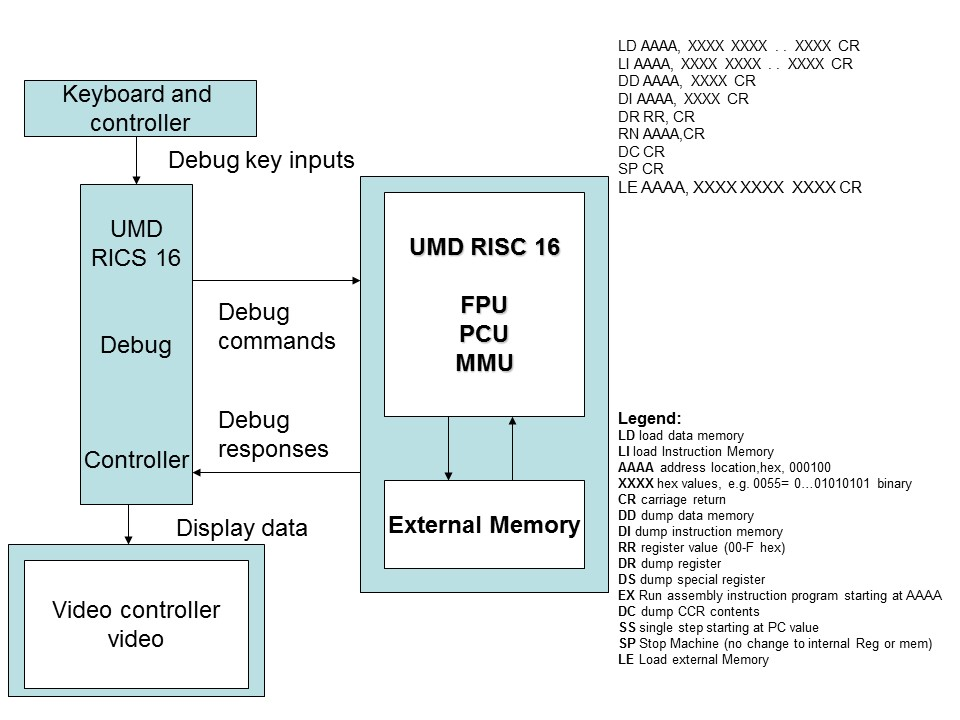
\includegraphics[width=0.7\textwidth]{images/RiscToplevel.jpg}}
  \caption{UMD RISC-16 Top Level I/O with debug conceptual architecture}
  \label{fig:RiscToplevel}
\end{figure}
\FloatBarrier

\begin{figure}[!htbp]
  \centering
      \fbox{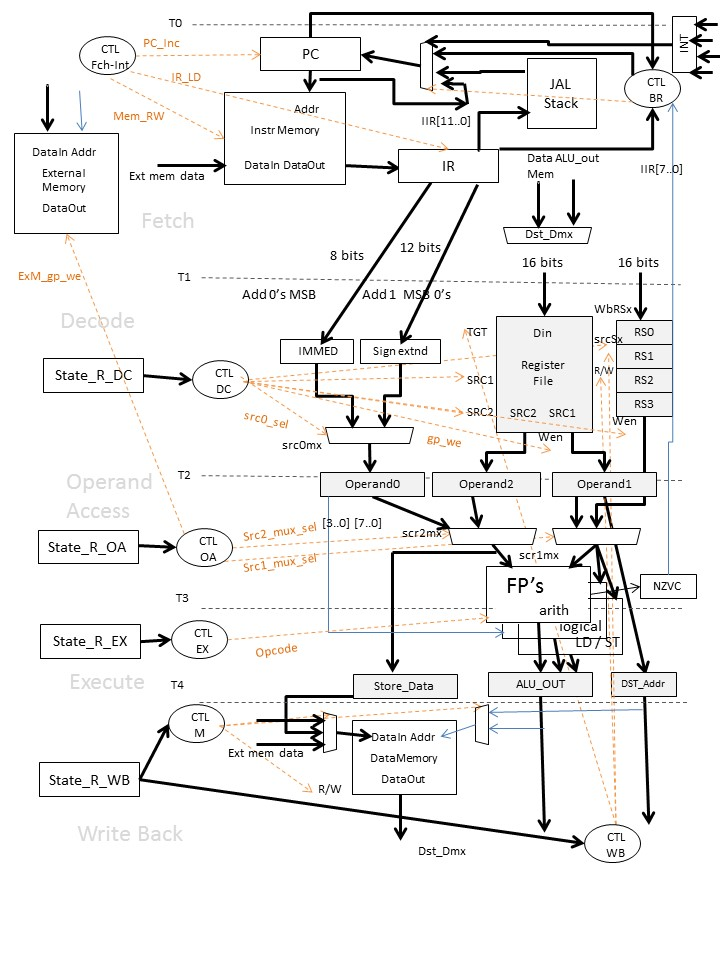
\includegraphics[width=0.7\textwidth]{images/UMDRISCLayout.jpg}}
  \caption{Notional UMD RISC-16 Full data path and control unit RTL architecture}
  \label{fig:UMDRISCLayout}
\end{figure}
\FloatBarrier

Interrupts will require you to choose a method for handling hardware generated signals (interrupts) and what they are to be used for. For example, interrupt one could be used to support the loading of data from the keyboard to the external memory. Another interrupt could be used to support the detection of some external hardware needing service.

\section{Procedure}

Follow the design procedure below to complete the lab. In this lab, you are required to create, document, and verify results of the test-benches and hardware test procedures you design and utilize in verifying and validating your design. Communicate which steps you were able to complete and the tests you used to ensure they operated as expected.

\begin{enumerate}

% Part 1
\item Table~\ref{tab:riscise} and Table~\ref{tab:risciseSI} shows the desired instruction set for the UMD-RISC 16 machine. You are required to add what is necessary for this lab at this current point. The shaded instructions are to be implemented for this lab to be successful. The LWVI, LWVD, SWED, SWEI and LWVS instructions will be necessary to demonstrate the functionality of your external memory unit that uses the Shadow registers. The INT instruction will require implementing additional data path connections, a 4 word vector address unit and additional controls. The INT instruction will require the addition of an additional control element at a minimum and methods for halting processing of instructions, saving processor state information (if needed), starting execution at a given vector address, and restarting the original halted instruction sequence upon completion of interrupt handling.

\begin{table}[!htbp]
\rowcolors{2}{gray!25}{white}
  \begin{center}
    \begin{tabular}{|c|l|l|}
       \hline
       \rowcolor{gray!50}
       \large{\textbf{OPCODES:}} & \large{\textbf{Operation:}} & \large{\textbf{Routine:}} \\
       \hline 
       \textbf{0000} & ADD  REG A, REG B & \specialcell{R[A] $\leftarrow$ R[A] + R[B] \\set status flags NZVC}  \\
       \textbf{0001} & SUB  REG A, REG B & \specialcell{R[A] $\leftarrow$ R[A] - R[B] \\set status flags NZVC}  \\
       \textbf{0010} & AND  REG A, REG B & \specialcell{R[A] $\leftarrow$ R[A] \& R[B] \\set status flags NZVC}  \\
       \textbf{0011} & OR   REG A, REG B & \specialcell{R[A] $\leftarrow$ R[A] $\mid$ R[B] \\set status flags NZVC}  \\
       \textbf{0100} & MOV  REG A, REG B & R[A] $\leftarrow$ R[B] \\
       \textbf{0101} & ADDI REG A, IMMED & \specialcell{R[A] $\leftarrow$ R[A] + IMMED \\set status flags NZVC}  \\
       \textbf{0110} & ANDI REG A, IMMED & \specialcell{R[A] $\leftarrow$ R[A] \& IMMED \\set status flags NZVC}  \\
       \textbf{0111} & SL   REG A, IMMED[0..3] & \specialcell{ R[A] $\leftarrow$  R[A\textless \textless IMMED] \\ zero fill LSB C and V affected}  \\
       \textbf{1000} & SR   REG A, IMMED[0..3] & \specialcell{R[A] $\leftarrow$ R[A\textgreater \textgreater IMMED] \\zero fill MSB}  \\
       \textbf{1001} & LW   REG A, IMMED[7..0] & R[A] $\leftarrow$ MEM[IMMED]  \\
       \textbf{1010} & SW   REG A, IMMED[7..0] & MEM[IMMED] $\leftarrow$ R[A]  \\
       \textbf{1011} & LWV  REG A, REG S, IMMED[7..0] & \specialcell{R[A] $\leftarrow$ ExMEM[R[S] + IMMED] \\when ID=00}  \\
       \textbf{1100} & SWV  REG A, REG S, IMMED[7..0] & \specialcell{ExMEM[R[S] + IMMED] $\leftarrow$ R[A] \\when ID=00}  \\
       \textbf{1101} & JAL  IMMED[16..0] & \specialcell{STK[SP+] $\leftarrow$ [PC],\\ PC $\leftarrow$ IMMED[16..0]}  \\
       \textbf{1110} & RTL & PC $\leftarrow$ STK[SP], SP $\leftarrow$ SP-1  \\
       \textbf{1111} & BRA MASK, IMMED[15..0] & \specialcell{PC $\leftarrow$ [PC]+ IMMED, \\if MASK \& NVZC is true}  \\
       \hline
    \end{tabular}
  \end{center}
  \caption{UMD RISC-16 Instruction Set Architecture}
  \label{tab:riscise}
\end{table}
\FloatBarrier


\begin{table}[!htbp]
\rowcolors{2}{gray!25}{white}
  \begin{center}
    \begin{tabular}{|c|l|l|}
       \hline
       \rowcolor{gray!50}
       \multicolumn{3}{|l|}{\LARGE{\textbf{Special Instructions:}}} \\
       \hline
       \large{\textbf{OPCODES:}} & \large{\textbf{Operation:}} & \large{\textbf{Routine:}} \\
       \textbf{1011} & \specialcell{LWVI REG A, REG S,\\ ID=10, IMMED[3..0]} & \specialcell{instmem[R[A]] $\leftarrow$ ExMEM[S[R] + IMMED]}  \\
       \textbf{1011} & \specialcell{LWVD  REG A, REG S,\\ ID=01, IMMED[3..0]} & \specialcell{datamem[R[A]] $\leftarrow$ ExMEM[S[R] + IMMED]}  \\
       \textbf{1011} & \specialcell{LWVS  REG A, REG S,\\ ID=11, IMMED[3..0]} & \specialcell{S[R] $\leftarrow$ R[A] + IMMED}  \\
       \textbf{1100} & \specialcell{SWED  REG A, REG S,\\ ID=01, IMMED[3..0]} & \specialcell{ExMEM[R[S] + IMMED] $\leftarrow$ DataMem[R[A]]}  \\
       \textbf{1100} & \specialcell{SWEI  REG A, REG S,\\ ID=10, IMMED[3..0]} & \specialcell{ExMEM[R[S] + IMMED] $\leftarrow$ InstructionMem[R[A]]}  \\
       \textbf{1100} & \specialcell{INT  REG A, REG S,\\ ID=11, IMMED[3..0]\\REG S = 11 enable\\REG S = 00  disable} & \specialcell{Interupt Enable/Disable\\ Bit[3..0] interrupt lines}  \\
       \hline
    \end{tabular}
  \end{center}
  \caption{UMD RISC-16 Special Instructions}
  \label{tab:risciseSI}
\end{table}
\FloatBarrier


% Part 2
\item Create new components for use in your project for special instructions external memory access and interrupt support.

Much of the remaining support elements will consist of registers, multiplexers, new control states, etc. to be utilized extended instructions and the interrupt operations.

% Part 3
\item Test your design by loading a program from your keyboard into your instruction memory and executing it.

% Part 4
\item Fully test your design. 

Develop a test procedure and demonstrate that you have faithfully implemented the ISA as indicated and that your machine is operating as pipelined processor.

Be sure to document your hardware test procedure and report results clearly.

\end{enumerate}

\section{Deliverables}

Please only print out your top level code and any new component code. A print out of all your code is not necessary. Please zip all VHDL files and UCF file and email to the \textbf{Instructor} and the \textbf{TA} with the filename \textbf{ECE368\_Project\_ Lab3\_Team\#.zip}.

Explain your testbench, print out your testbench results, and discuss the results you saw.

Likewise, explain your hardware test plan and procedures and any final results and/or problems you had. Be explicit; use detailed tables to describe what is being tested, what inputs are and what expected and measured outputs are and the result of the test.

Include any handwritten design flowcharts or pseudo code used in your lab report.

\section{Lab Report:}

Each lab group should prepare a lab report with the following information:
\begin{itemize}
  \item Follow the \textbf{CPE Laboratory Report Guidelines} for base format
  \item Machine RTL block level design
  \item VHDL component specification and schematic designs.
  \item VHDL system specification and resulting schematic design.
  \item Test plan design and test bench code
  \item Hardware test procedure used to verify your design
  \item Simulation results for your simple machine using a testbench (Prove it works).
  \item Schematic and UCF file for your simple machine.
  \item Conclusion needs to include a discussion of the learning utility of this lab and discussion of any issues you had with lab design and clarity.
  \item Reflection section discussing what you did well in your design, what you did not so good and why and what you plan to do to improve your design and design skills in the next lab and for the final project.
\end{itemize}

\section{Extra Credit:}

Dual pipeline operational. Two words in each phase of operation per cycle.

\section{Project Lab 3 Grade}

\begin{table}[!htb]
  \begin{center}
    \begin{tabular}[width=0.9\textwidth]{|l|c|l|}
       \hline
       Section & Value & Score\\
       \hline 
       \multicolumn{1}{|l}{\textbf{Procedure:}}  & -\textbf{40}- &\\
       \hline
       1. Implement Load Word Vector Instruction (LWVI) & 5 &\\
       \hline
       2. Implement Load Word Vector Data  (LWVD) & 5 &\\
       \hline
       3. Implement Load Word Vector Shadow Register (LWVS) & 5 &\\
       \hline
       4. Implement Store Word External from Data (SWED) & 5 &\\
       \hline
       5. Implement Store Word External Instruction (SWEI) & 5 &\\
       \hline
       6. Implement Interrupts (INT) & 5 &\\
       \hline
       7. Test loading a program from a keyboard and execute it & 5 &\\
       \hline
       8. Fully Test your Final Design & 5 &\\
       \hline 
       \multicolumn{1}{|l}{\textbf{Extra Credit:}}  & -\textbf{20}- &\\
       \hline
       1. Dual pipeline operational & 20 &\\
       \hline
       \multicolumn{1}{|l}{\textbf{Deliverables:}}  & -\textbf{40}- &\\
       \hline
       \multicolumn{1}{|l}{\textbf{Lab Report:}}  & -\textbf{20}- &\\
       \hline
       \hline
       \multicolumn{1}{|l}{Total} & \multicolumn{1}{c|}{100-120} &\\
       \hline
    \end{tabular}
  \end{center}
  \caption{Project Lab 3 Grade Breakdown}
\end{table}

\end{document}
